\documentclass[a4paper,11pt]{article}

\usepackage[utf8]{inputenc}  
\usepackage[brazil]{babel}

\usepackage[margin=2.5cm]{geometry}  
\usepackage{graphicx}
\linespread{1.3}
\usepackage{amssymb}
\usepackage{palatino,euler}   

\title{MAC 300: EP3: Matrizes ortogonais e o problema de quadrados mínimos} 
\author{Bruno Ferrero}
\date{NUSP: 3690142}

\begin{document}

\maketitle

\section*{Fatoração QR}
O objetivo é fatorar $ A  \in  \mathbb{R}^{mxn} $, tal que $A = QR$, em que $Q$ é uma matriz ortogonal e $R$ uma matriz triangular superior. O método implementado utiza as matrizes de reflexões (refletores ou \textit{Householder transformations}) para gerar a matriz ortogonal. O algoritmo foi implementado baseado no \textit{Fundamentals of Matrix Computations, 2Ed - David Watkins}, com adaptações para que ele fosse orientado à linhas. 

\section*{Arquivos entregues}

Além dos casos testes (\texttt{caso0*.dat}):

\begin{itemize}
\item \texttt{qr.c} : Código fonte \texttt{C}.
\item \texttt{tests.m} : script para \textit{matlab}. Com ele foram gerados todos os testes utilizados neste EP.
\item \texttt{relatorio\_ep3.tex} : fonte do relatório.

Para executar:
\begin{itemize}
\item[\$] \texttt{gcc -Wall -ansi -pedantic qr.c -o qr.out}
\item[\$] \texttt{./qr.out caso03.dat}
\end{itemize}
\end{itemize}

A matriz $A$ e o vetor $b$ são lidos do arquivo \texttt{.dat} e o resultado ($x$) de $Ax=b$ é impresso na tela.

\section*{Testes}
Foram gerados 4 casos para teste utilizando o script \texttt{testes.m}. Para testar os resultados utilizei o resultado $x$, que é impresso na tela ao executar o EP no matlab e verifiquei a igualdade do sistema $Ax=b$.
\begin{enumerate}
\item O primeiro caso resolve o sistema $Ax=b$ para uma matriz $A$ e um vetor $b$ arbitrários. 

\item No segundo caso gera-se uma matriz $Q$ ortogonal e uma matriz $R$ triangular superior. Obtêm-se $A$ pela multiplicação das duas anteriores. $b$ é um vetor de inteiros gerado aleatóriamente. O tempo de execução da fatoração da matriz $A$ de tamanho $n=100$ foi $0.005186$ segundos. 

\item O terceiro caso, a matriz $A$ é gerada da mesma forma que no caso anterior, no entanto, é gerado uma matriz de tamnho $n=1000$. Neste caso, a fatoração $QR$ levou $4.735840$ segundos para executar. Ou seja, levou em torno de $10^3$ vezes mais tempo do que no caso anterior. 

\item O quarto caso (Figura \ref{fig}), simula um conjunto de medidas que são armazenadas em um vetor $b$. A ideia é ajustar um polinômio de grau $1$ à curva de medidas. A base do polinômio é $(t^0 , t^1)$. Os coeficiente serão dados por $x$, que é solução de $Ax=b$.

\end{enumerate}

\begin{center}
\begin{figure}[h]
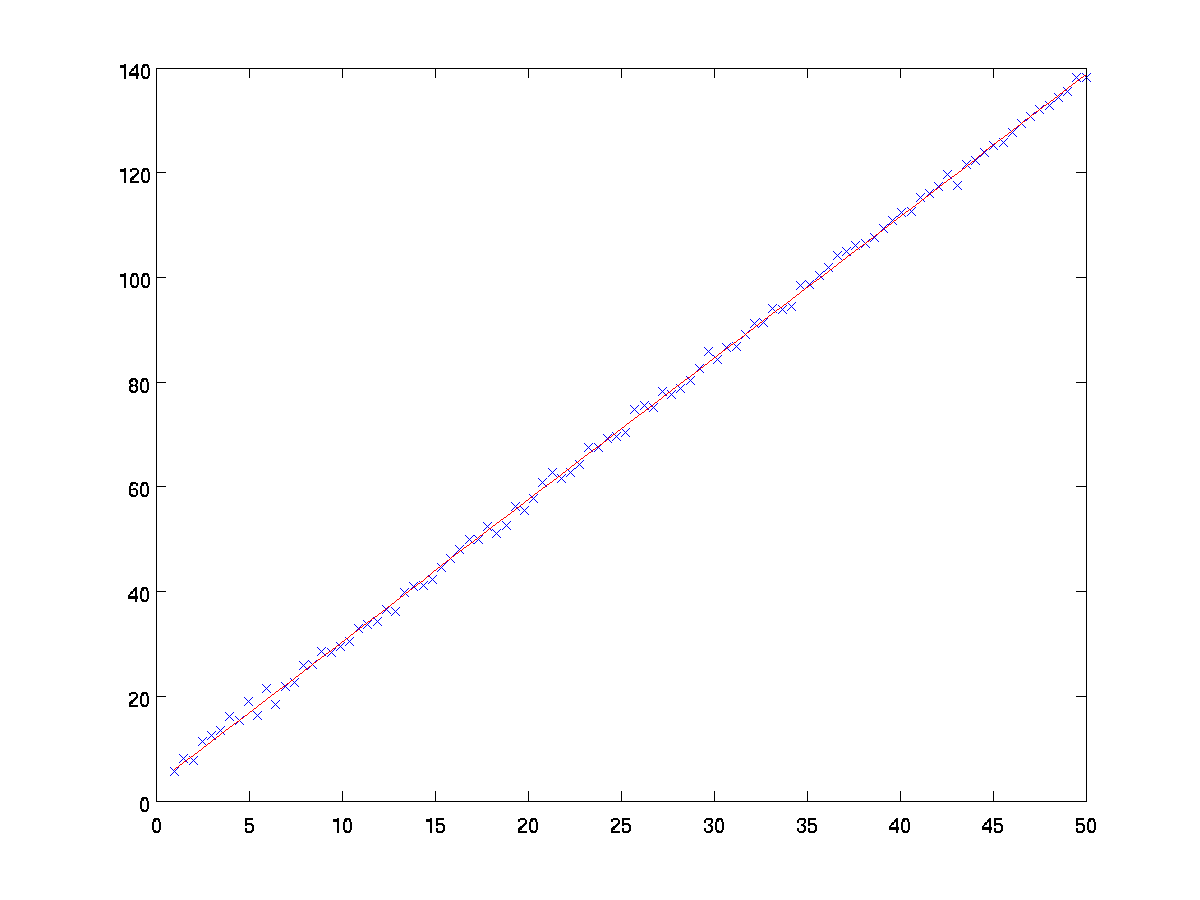
\includegraphics[width=15cm,keepaspectratio]{curve_fit.png}
\caption{A cor azul é o dado original ($y$) e vermelho a reta ajustada pelo polinômio $p(t) = 3.317559 + 2.707609t;$. Os coeficientes do polinômio $(x_0,x_1)$ foram calculados resolvendo-se o sistema $Ax=b$. }
\label{fig}
\end{figure}
\end{center}


\end{document}
